\documentclass[handout]{beamer}

\title{Generating PDFs With (and Without) Python}
\author{David Fischer}
\date{August 27, 2015}

%% Beamer Themes
\usetheme{Berlin}
\usecolortheme{dove}
\usefonttheme{serif}

%% Packages
% Pygments must be accessible to use minted and --shell-escape
%  must be used with pdflatex
\usepackage{minted}
\usepackage{hyperref}
\usepackage[font=scriptsize,labelformat=empty]{caption}


\setbeamertemplate{footline}{
  \hspace*{.2cm}
  \scriptsize{
    \insertshorttitle
    \hspace*{50pt}
    \hfill
    \insertframenumber/\inserttotalframenumber
    \hspace*{.2cm}
  }
  \vspace{9pt}
}


\begin{document}

\maketitle

\begin{frame}
\frametitle{What are PDFs?}
  {\huge Document Presentation Format}
\end{frame}


\begin{frame}
  \begin{itemize}
    \item Precisely lays out elements on a page
    \item Has a concept of the size of the paper
    \item Cross platform
    \item Standardized
  \end{itemize}
\end{frame}


\begin{frame}
\frametitle{}
  {\huge Anything destined for a printer should probably be a PDF}
\end{frame}


% Fragile is required for syntax highlighting
\begin{frame}[fragile]
\frametitle{ReportLab}

{\scriptsize
\begin{minted}{python}
import reportlab
from reportlab.platypus import SimpleDocTemplate, Paragraph
from reportlab.lib.styles import getSampleStyleSheet, ParagraphStyle
from reportlab.lib.units import inch
from reportlab.lib.pagesizes import letter

import io


buf = io.BytesIO()

# Setup the document with paper size and margins
doc = SimpleDocTemplate(
    buf,
    rightMargin=inch/2,
    leftMargin=inch/2,
    topMargin=inch/2,
    bottomMargin=inch/2,
    pagesize=letter,
)
\end{minted}
}

\end{frame}


\begin{frame}[fragile]
\frametitle{ReportLab (continued)}

{\scriptsize
\begin{minted}{python}
# Styling paragraphs
styles = getSampleStyleSheet()

# Write things on the document
paragraphs = []
paragraphs.append(
    Paragraph('This is a paragraph', styles['Normal']))
paragraphs.append(
    Paragraph('This is another paragraph', styles['Normal']))
doc.build(paragraphs)

# Write the PDF to a file
with open('my.pdf', 'w') as fd:
    fd.write(buf.getvalue())
\end{minted}
}

\end{frame}



\begin{frame}[fragile]
\frametitle{Sphinx and ReStructuredText}

{\scriptsize
\begin{minted}{rst}
.. index.rst
Heading
=======

This is a paragraph.

This is a `link <http://example.org>`_

Subheading
----------

.. This is a table of contents

.. toctree::
   :maxdepth: 2

   01-first-import
\end{minted}
}
\end{frame}


\begin{frame}
  \begin{figure}[p]
    \centering
    \fbox{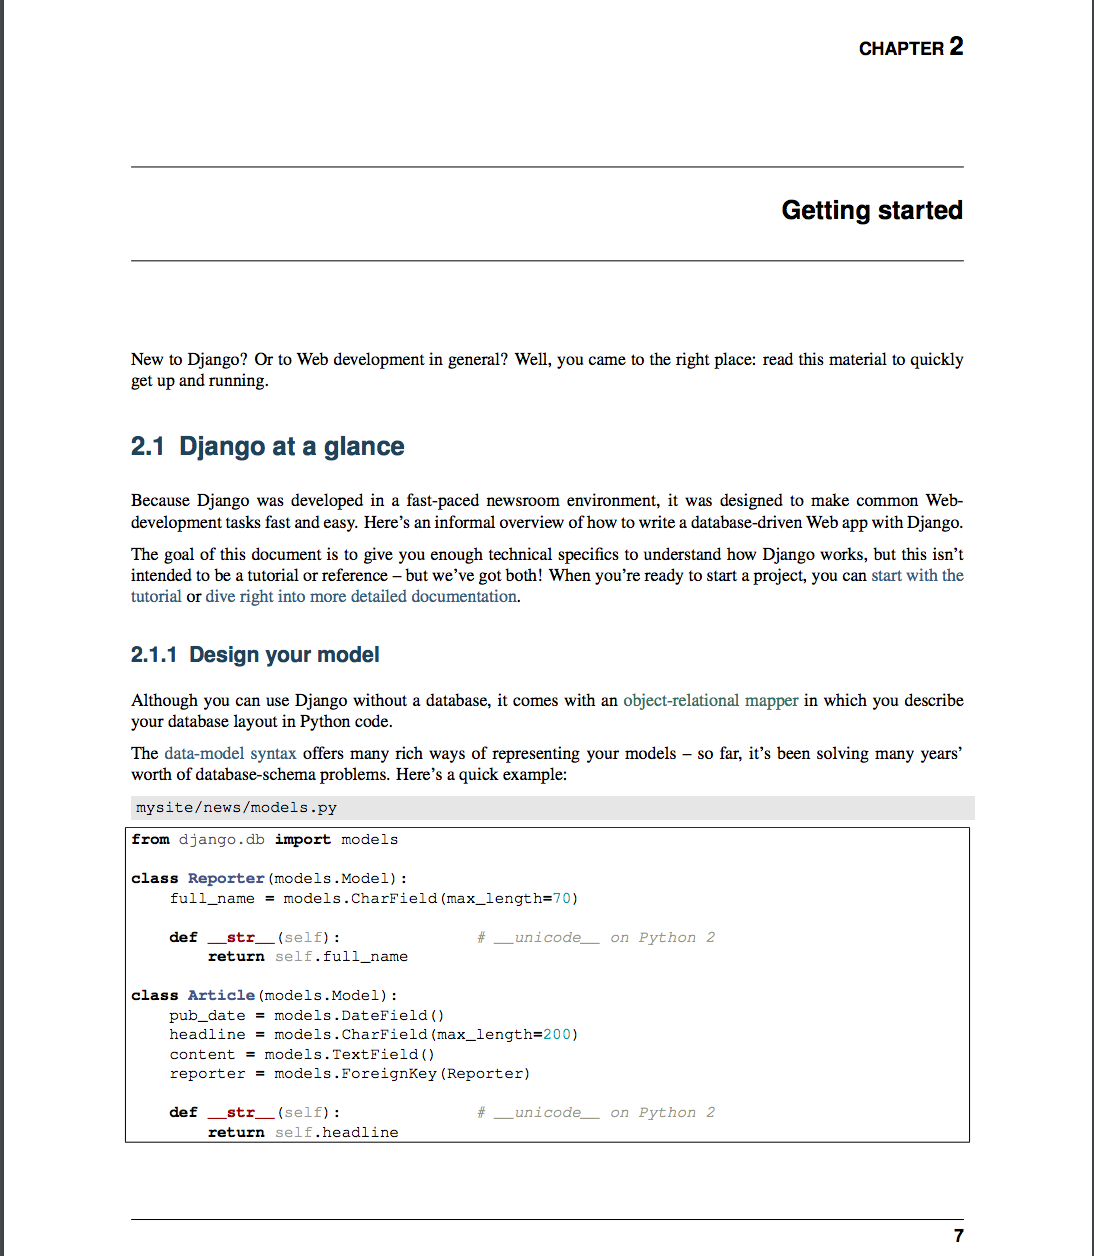
\includegraphics[height=0.7\paperheight]{includes/django-docs.png}}
    \caption{Django documentation rendered as a PDF by Sphinx}
  \end{figure}
\end{frame}


\begin{frame}[fragile]
  \frametitle{\LaTeX}

{\scriptsize
\begin{minted}{tex}
\documentclass{article}
\begin{document}
  % Use your favorite templating engine
  % and generate your PDF with the well used pdflatex
  {\small This is some small text }

  % This presentation was created with LaTeX
\end{document}
\end{minted}
}

\end{frame}


\begin{frame}
  \frametitle{Others}

  \begin{itemize}
    \item \href{http://www.xhtml2pdf.com/}{XHTML2PDF}, \href{http://wkhtmltopdf.org/}{wkhtmltopdf}, \href{http://phantomjs.org/}{PhantomJS} (HTML)
    \item \href{https://inkscape.org/}{Inkscape} (SVG)
    \item \href{https://github.com/ccnmtl/fdfgen}{FDFGen} (PHP with a Python port)
  \end{itemize}
\end{frame}


\begin{frame}
\frametitle{Resources}
  \begin{itemize}
    \item {\small \href{http://www.reportlab.com/}{http://www.reportlab.com/}}
    \item {\small \href{http://www.latex-project.org/}{http://www.latex-project.org/}}
    \item {\small \href{http://sphinx-doc.org/}{http://sphinx-doc.org/}}
    \item {\small \href{http://docutils.sourceforge.net/}{http://docutils.sourceforge.net/}} (reST)
    \item {\small \href{https://docs.djangoproject.com/en/dev/howto/outputting-pdf/}{https://docs.djangoproject.com/en/dev/howto/outputting-pdf/}}
  \end{itemize}
\end{frame}


\end{document}
